\section {Vergleich reaktive \& imperative Anwendung}
\label{section:vergleich_reaktiv_imperativ}
Um zu prüfen, ob Leistungsfähigkeit und Skalierbarkeit einer reaktiven Anwendung tatsächlich die einer traditionellen, imperativen Anwendung
übertrifft, werden in diesem Kapitel beide Ansätze hinsichtlich verschiedener Metriken in einem festen Zeitintervall miteinander verglichen.
//TODO auslagern in kapitel testmethodik und kapitel ergebnisse?
Dafür werden sowohl die reaktive, als auch die nicht-reaktive Anwendung zwei Lasttests unterzogen: //TODO: Testreihen?
\begin{enumerate}
	\item Abfrage von Statische Daten
	\item Abfrage von dynamischen Daten mit Datenbankanbindung
\end{enumerate}
Dabei wird eine Reihe an Lasten bzw. \textit{workloads} von einem Client-Host generiert und über eine feste Dauer in kleinen Zeitinvervallen
an einen ausgewählten HTTP-Endpunkt der Anwendung gesendet.
In dieser Zeit wird das Zeitinvervall vom Starten der Anwendung bis zur Beantwortung der ersten Anfrage,
der benötigte Arbeitsspeicher und CPU-Auslastung des Prozesses, der Durchsatz, sowie die Latenz gemessen.

Für Container- und Cloud-Umgebungen eignen sich, primär aus Kostengründen, Anwendungen die, statt auf hohen Durchsatz und lange Laufzeiten, auf
schnelle Startzeiten und geringen Ressourcenverbrauch setzen.
Aus diesem Grund werden die beiden Anwendungen sowohl im \textit{JVM mode} als auch im \textit{native mode}
(siehe \ref{section:java_tooling}) den Lasttests unterzogen. Ingesamt ergeben sich also 4 Testszenarien.


\subsection{Implementierung \& Systemaufbau}
\label{section:implementierung}
Die beiden Anwendungen implementieren mit dem Quarkus-Framework jeweils eine simple REST-Schnittstelle mit HTTP-CRUD Methoden
und einer angebundenen PostgreSQL-Datenbank.
Dabei ist vorallem die HTTP-Schicht von Interesse. Die HTTP-Unterstützung von Quarkus basiert auf einem reaktiven, nicht-blockierenden
Unterbau: der Vert.x Engine.
Jede HTTP-Anfrage wird auf einem der \textit{event-loop threads} bzw. \textit{IO threads}
\footnote{Deren Anzahl hängt von der Anzahl der CPU-Kerne ab}
verarbeitet und durch eine Routing-Schicht an den Anwendungscode weitergeleitet.
Je nachdem welcher Ansatz zur Implementierung des jeweiligen HTTP-Endpunktes gewählt wurde,
wird der abzuarbeitende Code dann auf einem blockierenden \textit{worker thread} aus dem \textit{worker thread pool}
\footnote{Auch als \textit{Dispatch} bezeichnet} (Servlet, JAX-RS) oder einem der
\textit{IO threads} (Reactive Routes, Reactive Resteasy) ausgeführt.
Die \textit{IO threads} sind dafür zuständig alle IO-Operationen asynchron auszuführen und die jeweiligen EventListener bzw. Subscriber
auszulösen sobald die Operationen abgeschlossen sind.
\newpage
\begin{figure}[h!]
	\centering
	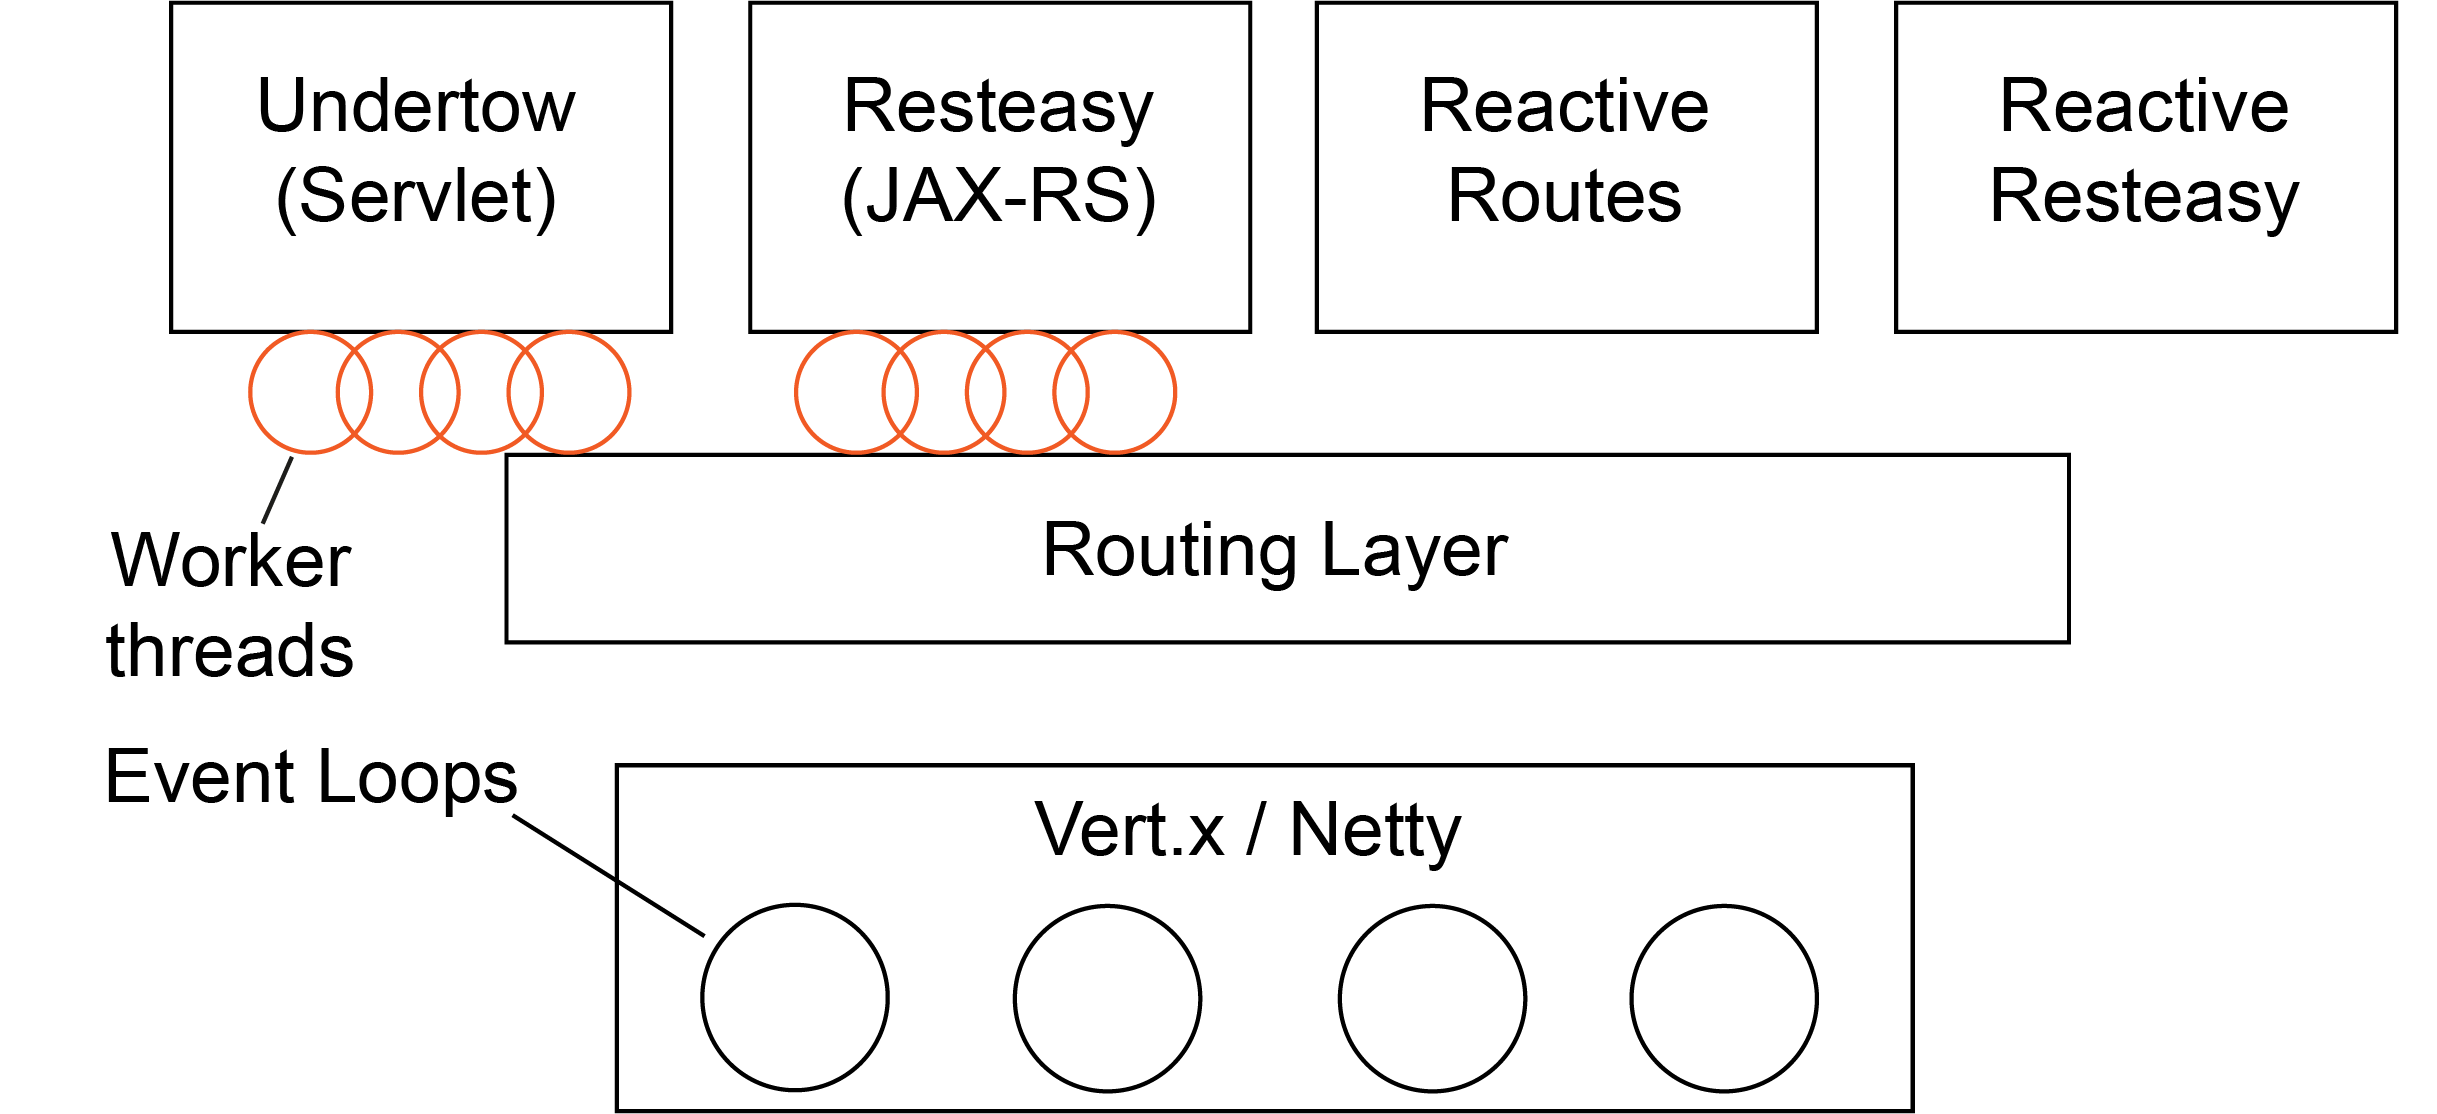
\includegraphics[width=1.0\textwidth]{Quarkus_HTTP_Layer}
	\caption{Quarkus HTTP-Schicht \parencite{QuarkusReactiveRoutes}}
\end{figure}

Damit sich beide Anwendungen nahe an einer realen Java-EE REST-API orientieren, haben
sie (zusätzlich zu den grundlegenden Abhängigkeiten des Quarkus-Frameworks) folgende Projekt-Abhängigkeiten:
\begin{enumerate}
	\item JAX-RS Implementierung
	\item JSON Unterstützung
	\item Datenbanktreiber
	\item JPA Implementierung
\end{enumerate}

Diese Abhängigkeiten wurden vom Quarkus Maven-Repository sowohl in blockierender,
als auch in nicht-blockierender, reaktiver Form bereitgestellt: \parencite{MavenQuarkusIO}
% space between the text and the left/right border of its containing cell is set to 18 pt
\setlength{\tabcolsep}{18pt}
% the height of each row is set to 1.5 relative to its default height
\renewcommand{\arraystretch}{1.5}
\begin{table}[ht!]
	\centering
	\begin{tabular}{| c | c | c |}
		\hline
		                 & Blockierend      & Nicht-blockierend (reaktiv) \\
		\hline
		JAX-RS           & Resteasy         & Resteasy Reactive           \\
		\hline
		JSON             & Resteasy-Jackson & Resteasy-Reactive-Jackson   \\
		\hline
		Datenbanktreiber & JDBC-Postgresql  & Reactive-Pg-Client          \\
		\hline
		JPA-/ORM         & Hibernate-ORM    & Hibernate-Reactive          \\
		\hline
	\end{tabular}
	\caption{Tabelle mit den Abhängigkeiten beider Applikationen}
	\label{table:dependencies}
\end{table}
TODO add some text to listings
\begin{lstlisting}[caption=Update Methode der reaktiven Anwendung, language=Java, captionpos=b, label=lst:update_reactive]
    @PUT
    @Path("{id}")
    public Uni<Response> update(Long id, Fruit fruit) {
        if (fruit == null || fruit.getName() == null) {
            return Uni.createFrom().item(Response.status(422).build());
        }
        return fruitRepository.findById(id).onItem()
        .ifNotNull().invoke(storedFruit -> storedFruit.setName(fruit.getName())
        ).call(storedFruit -> fruitRepository.update(storedFruit))
                .onItem().ifNotNull().transform(storedFruit ->
                 Response.ok(storedFruit).build())
                .onItem().ifNull().continueWith(Response.status(Status.NOT_FOUND).build());
    }
   \end{lstlisting}
\begin{lstlisting}[caption=Update Methode der nicht-reaktiven Anwendung, language=Java, captionpos=b, label=lst:update_blocking]
    @PUT
    @Path("/{id}")
    public Response update(Fruit fruit, @PathParam("id") Long id) {
        if (fruit == null || fruit.getName() == null) {
            return Response.status(422).build();
        }
        Fruit storedFruit = fruitRepository.findById(id);
        if (storedFruit == null) {
            return Response.status(Response.Status.NOT_FOUND).build();
        }
        storedFruit.setName(fruit.getName());
        fruitRepository.update(storedFruit);
        return Response.status(Response.Status.OK).build();
    }
   \end{lstlisting}

Der Projekt-Code dieser Arbeit kann vom Gitlab-Server der Ostfalia unter
\url{//TODO Ostfalia Gitlab link?} eingesehen und abgerufen werden.

\subsection{Testumgebung}
\label{section:testumgebung}
Für die Testumgebung werden zwei Systeme benötigt: der Client-Host und der Server-Host.
Dabei muss es sich um UNIX-Systeme handeln, da eine einige der verwendeten Werkzeuge nur
auf diesen Systemen verfügbar sind.
Zudem müssen beide Systeme per SSH von einem (idealerweise vorhandenem) dritten System, dem User-Host
\footnote{Dies kann allerdings auch der Client-Host selber sein}
erreichbar sein, damit dieses den Testablauf in der korrekten Abfolge ausführen kann.
Der Einfachheit halber empfiehlt es sich, dass sich alle Geräte im gleichen Netzwerk befinden.
//TODO warum -> aufwendige netzwerkkommunikation ?
Beiden Anwendungen verwenden Version 1.12.1 des Quarkus Frameworks.

Um eine reproduzierbare Anwendungsumgebung und Ressourcenallokation zu ermöglichen, laufen beide Anwendungen auf dem Server-Host in
jeweils einem Docker-Container mit fest definierten Ressourcen:
\begin{itemize}
	\item Nutzung von 4 CPU-Kernen
	\item 1024 MB RAM
	\item 256 MB Heap Größe für den Java-Prozess
	      \footnote{Seit Java 10 wird automatisch ~1/4 des Speicher Limits des Containers genutzt \parencite{Java10ReleaseNotes}}
\end{itemize}
Der jeweilige Docker-Container für die Postgresql-Datenbank allokiert:
\begin{itemize}
	\item 4 CPU-Kerne
	\item 2048 MB RAM
\end{itemize}
//TODO: Größe von Event-Loop Thread Pool (4/8) und Worker Thread Pool(20) in Vert.x nennen und begründen warum Event-Loop Thread Pool Size explizit
gesetzt werden muss (Vert.x Version )
//TODO: Readme in Java-Projekt anpassen und Hinzufügen das Event-Loop Thread Pool Size explizit gesetzt werden muss da Vert.x die Limitierungen d
//TODO: Komplett neue Tests (diesmal als Testreihe) durchführen durch Korrektur der Event-Loop Thread Pool Size
des Containers nicht berücksichtigt
Die Anwendung, die auf dem Client-Host die \textit{work load} für die beiden zu testenden Anwendungen generiert,
nutzt in dieser Testumgebung 4 Threads.
Welche Laufzeitumgebungen und Tools für die Tests auf den jeweiligen Hosts vorhanden sein müssen,
wird in der Readme.md-Datei des Projektverzeichnisses genau beschrieben.
Da die Messergebnisse je nach verwendeter Hardware der Client- und Server-Hosts durchaus variieren können werden im Folgenden
die Systemspezifikationen der verwendeten Systeme des Authors gelistet:
\begin{table}[ht!]
	\centering
	\begin{tabular}{| c | c |}
		\hline
		Server-Host                                                  \\
		\hline
		CPU's          & AMD Ryzen 7 2700x eight-core processor x 16 \\
		\hline
		RAM            & 16GB                                        \\
		\hline
		Speicher       & 1,5 TB                                      \\
		\hline
		Betriebssystem & Fedora 34 (Workstation Edition)             \\
		\hline
		Kernel         & Linux version \verb|5.12.14-300.fc34.x86_64|    \\
		\hline
	\end{tabular}
	\caption{Systemspezifikationen der verwendeten Server-Maschine}
	\label{table:system_host}
\end{table}

\begin{table}[ht!]
	\centering
	\begin{tabular}{| c | c |}
		\hline
		Client-Host                                               \\
		Hardware       & Acer Aspire VN7-591G                     \\
		\hline
		CPU            & Intel® Core™ i5-4210H CPU @ 2.90GHz × 4  \\
		\hline
		RAM            & 8GB                                      \\
		\hline
		Speicher       & 500 GB                                   \\
		\hline
		Betriebssystem & Fedora 34 (Workstation Edition)          \\
		\hline
		Kernel         & Linux version \verb|5.12.14-300.fc34.x86_64| \\
		\hline
	\end{tabular}
	\caption{Systemspezifikationen der verwendeten Client-Maschine}
	\label{table:system_client}
\end{table}

\subsection{Testvorgehen / Testaufbau}
\label{section:vorgehen}
Der im Folgenden erläuterte Versuchsaufbau basiert auf einer, vom Autor erweiterten, Architektur die vom Quarkus-Entwicklerteam
zur Erstellung von verschiedenen Benchmarks für den Quarkus Technologie-Stack genutzt wurde.
\parencite{QuarkusBlog, QuarkusJohnaohara}

Um den gesamten Versuchsablauf zu automatisieren und über mehrere Server zu steuern wird ein Tool namens qDup eingesetzt.
Damit können Shell-Kommandos als Skripte gruppiert, und verschiedenen Hosts je nach Rolle zugewiesen werden.
\footnote{Die qDup Skripte mit dem gesamten Testablauf können im Verzeichnis \textit{/scripts/qDup} des Quellcodeverzeichnisses eingesehen und
	angepasst werden.}
Um dem Ablauf korrekt zu steuern werden Signale definiert die ein Host sendet, und auf die die anderen Hosts warten um ihrerseits
weitere Skripte auszuführen.
\footnote{Beispielsweise sollte der Server-Host erst anfangen den Java-Prozess zu überwachen, sobald der Client-Host die \textit{workload}
	generiert und nicht bereits davor}


Wie bereits in \ref{section:testumgebung} erwähnt, nutzt qDup SSH um mit den jeweiligen Servern zu kommunizieren.

Im ersten Schritt \textit{build applications} wird auf dem Server-Host das Quellcodeverzeichnis geklont und beide Anwendungen werden gebaut
(je nach Test entweder als uber-jar (//TODO: Warum Uber-Jar) oder als \textit{native executable}). Anschließend wird über ein JavaScript-Skript,
welches in der Laufzeitumgebung Node.js läuft, das durchschnittliche Zeitintervall zwischem dem Start einer Anwendung bis
zur Verarbeitung der ersten Anfrage gemessen
(\textit{Mean Start Time to First Request}). Darüber hinaus werden die Docker-Container der Datenbank
\footnote{Nur beim Test mit dynamischen Daten} und der beiden REST-APIs gebaut.

Beim zweiten Schritt \textit{run applications} wird der Docker-Container der jeweiligen Anwendung gestartet und anschließend signalisiert,
dass die Anwendung nun bereit ist.
Daraufhin wird auf dem Client-Host das Skript \textit{generate load} gestartet.
Die \textit{workload} ist hier definiert als die Anzahl der, an den Server-Host, versendeten \textit{HTTP-Anfragen pro Sekunde}.
Für das Generieren und Übermitteln der \textit{workload} wird das Werkzeug \textit{wrk2} genutzt, welches das
bewährte HTTP-Benchmarking Tool \textit{wrk} um folgende Funktionen erweitert:
\begin{enumerate}
	\item Konstanter \textit{workload} Durchsatz
	\item Korrekteres Messverfahren der Antwort-Latenz //TODO: Warum ? Erklären Unterschied Latenzmessung
	\item Exaktes Messen durch \Glsuseri{hdrHistogramm}
\end{enumerate}\parencite{Wrk2, Wrk}

Pro Test werden Benchmarks für eine ganze Reihe an \textit{workloads} gemessen.
Jede \textit{workload} wird über einen Zeitraum von 60 Sekunden über 100 offene HTTP-Verbindungen an den Server-Host übermittelt.
In den Tests nutzt \textit{wrk2} für das Generieren und Übermitteln der \textit{workload}, sowie das Messen der Antwortszeit
4 Threads.

Damit der Anwendungscode des angesteuerten HTTP-Endpunkts durch den JIT-Compiler der JVM optimiert wird,
findet pro \textit{workload} vor der eigentlichen Mess-Phase eine identische Warmup-Phase statt.

Listing \ref*{lst:generateLoad} zeigt den Aufruf von \textit{wrk2} mit den beschriebenen Parametern in der Warmup- und Mess-Phase,
\verb|${RUN_RATE}| enthält die \textit{workload}

\begin{lstlisting}[caption=Auszug des qDup Skripts generate load, captionpos=b, label=lst:generateLoad]
    - signal: ${{RUNTIME.name}}-${{RUN_RATE}}-WARM-UP-START
    - sh: wrk -t 4 -c 100 -d 60s -R ${{RUN_RATE}} ${{TEST_DYNAMIC_ENDPOINT}} > ${{CLIENT_FILE_PATH}}/output/${{RUNTIME.name}}-${{RUN_RATE}}-WARM-UP.wrk2.out
    - signal: ${{RUNTIME.name}}-${{RUN_RATE}}-WARM-UP-END
    - sh: sleep 5s
    - signal: ${{RUNTIME.name}}-${{RUN_RATE}}-MEASURE-START
    - sh: wrk -t 4 -c 100 -d 60s -R ${{RUN_RATE}} --latency ${{TEST_DYNAMIC_ENDPOINT}} > ${{CLIENT_FILE_PATH}}/output/${{RUNTIME.name}}-${{RUN_RATE}}-MEASURE.wrk2.out
    - signal: ${{RUNTIME.name}}-${{RUN_RATE}}-MEASURE-END
   \end{lstlisting}

Die Ausgabe von wrk enthält Informationen zur \Gls{latenz}\footnote{Pro verwendetem Thread und Gesamt},
zum \Gls{durchsatz} und der \Gls{perzentile} der \Gls{latenz} (durch ein \Gls{hdrHistogramm} dargestellt).
Listing \ref*{lst:wrk-listing} zeigt die umgeleitete Ausgabe von \textit{wrk} ohne die genaue Darstellung der Perzentile.

\begin{lstlisting}[caption=Beispiel für Ausgabe von wrk,captionpos=b, label=lst:wrk-listing]
    Running 1m test @ http://erik-pc.local:8080/greeting/Bob
    4 threads and 100 connections
    Thread calibration: mean lat.: 310.434ms, rate sampling interval: 1047ms
    Thread calibration: mean lat.: 330.365ms, rate sampling interval: 1127ms
    Thread calibration: mean lat.: 298.671ms, rate sampling interval: 994ms
    Thread calibration: mean lat.: 333.465ms, rate sampling interval: 1123ms
    Thread Stats   Avg      Stdev     Max   +/- Stdev
      Latency     1.76s   738.93ms   4.12s    62.98%
      Req/Sec    28.58k   633.82    30.09k    66.49%
    6839722 requests in 1.00m, 476.17MB read
   Requests/sec: 113929.77
   Transfer/sec:      7.93MB
   \end{lstlisting}\footnote{Die Resultate der Tests sind auch im Quellcodeverzeichnis unter \textit{\/results} zu finden}

Bevor die Warmup-Phase und die Belastungs-Phase mit \textit{wrk} vom Client-Host ausgeführt werden, wird dem Server-Host signalisiert, dass
er das Skript \textit{capture platform stats} ausführen soll.
In diesem Skript wird die Observation des Anwendungs-Prozesses durch das Kommandozeilenprogramm \textit{top} gestartet.
\textit{Top} wird dabei im Batch-Modus gestartet mit einer Wiederholrate von einer Sekunde.

Die Prozess-Zeile der Ausgabe von \textit{top} enthält eine Vielzahl an Informationen zu dem beobachteten Prozess, von besonderem
Interesse sind hierbei die CPU-Auslastung und der verwendete Arbeitsspeicher des Prozesses.

\begin{lstlisting}[language=sh, caption=Auszug des qDup Skripts capture-platform-stats, captionpos=b]
    - wait-for: ${{RUNTIME.name}}-${{RUN_RATE}}-WARM-UP-START
    - sh: top -b  -d 1 -p ${{RUN.JAVA_APP_PID}} | grep java > ${{SERVER_FILE_PATH}}/output/${{RUNTIME.name}}-${{RUN_RATE}}-WARM-UP-top.out &
    - sh: export TOP_PID=$!
    - wait-for: ${{RUNTIME.name}}-${{RUN_RATE}}-WARM-UP-END
    - sh: kill -9 $TOP_PID
    - wait-for: ${{RUNTIME.name}}-${{RUN_RATE}}-MEASURE-START
    - sh: top -b  -d 1 -p ${{RUN.JAVA_APP_PID}} | grep java > ${{SERVER_FILE_PATH}}/output/${{RUNTIME.name}}-${{RUN_RATE}}-MEASURE-top.out &
    - sh: export TOP_PID=$!
    - wait-for: ${{RUNTIME.name}}-${{RUN_RATE}}-MEASURE-END
    - sh: kill -9 $TOP_PID
  \end{lstlisting}

Im letzten Schritt werden alle Ausgaben über SSH vom Client- und Server-Host auf den User-Host, welches das qDup Skript ausgeführt hat, kopiert.

\begin{figure}[h!]
	\centering
	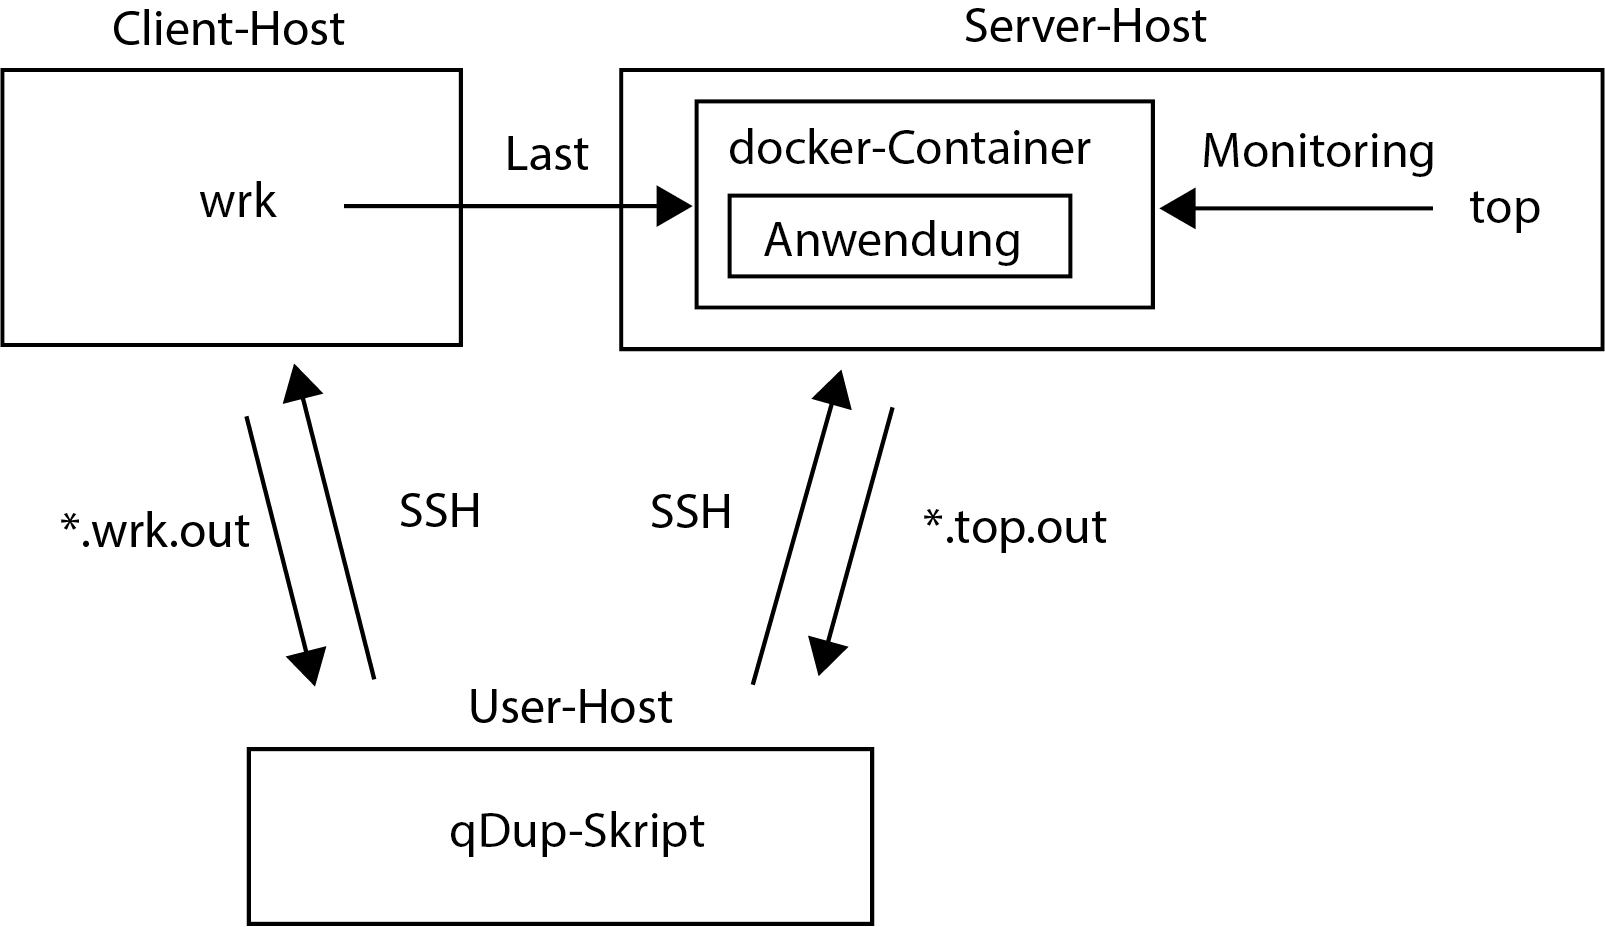
\includegraphics[width=0.8\textwidth]{Testaufbau}
	\caption{Testaufbau}
\end{figure}

In einem \verb|.sh|-Skript werden anschließend die Daten über ein Java-Skript, das mit dem Tool \textit{JBang} ausgeführt
wird \footnote{JBang erlaubt das direkte Ausführen von .java Dateien},
geparsed und die relevanten Daten bezüglich des Durchsatzes, Speicherverbrauches und CPU-Auslastung ermittelt.
Diese werden dann für die visuelle Darstellung in eine \verb|.json|-Datei geschrieben.
TODO genauer das filtern erklären (welcche sind die relevanten daten und wwas wird gefiltert)
Zu guter Letzt werden die aufbereiteten Daten durch die Node.js-Bibliothek \textit{d3node-linechart} in Form von Graphen visuell dargestellt.

\subsection{Test: Statische Daten}
\label{section:statische_daten}
TODO: Arbeit formattieren und vorherige TODOs abarbeiten bevor anfangen
\subsubsection{Systemablauf}
//TODO: Grafik ähnlich zu Grafik in Implementierung aber mit Threadwechseln und exemplarisch mhrere Threads zeigen
(auch angeben wie Ergebnisse mit komplizierteren Queries aussehen könnten)
\subsubsection{Resultate}

\subsection{Test: Datenbankzugriffe}
\label{section:datenbankzugriffe}

\subsubsection{Systemablauf}
//TODO: Grafik ähnlich zu Grafik in Implementierung aber ohne Threadwechsel dafür Main-Thread mit dahinterliegender Datenbank,
das Nicht BLockieren bzw. Asynchronität verdeutlichen

\subsubsection{Resultate}

//auch erwähnen dss beide paradigmen gemischt werden können, und vert.x dann entweder die anfrage an den worker thread pool dispatched
// (auch mit kosten verbunden)
// oder auf dem io thread ausführt also muss nicht komplett reaktiv oder blockierend sein x
\subsection{Auswertung}

\label{section:auswertung}